
\section{Estimating the Spatial Closure from the HO Solution}
\label{sec:spat_clos}

This sections describes an alternative spatial closure to the LO equations based on 
a parametric relation from the HO solution. 
After approximating the angular consistency terms in the time-discretized moment equations, 
there is still more unknowns than equations, for each spatial
cell and half range; an extra equation relating the spatial moments and face values is
needed.  The HO solution can be used to estimate the relation so that, upon nonlinear
convergence, the LO moments will exactly preserve the HO moments.  The only discretization
error is then what errors were introduced into the HO equations.
In the remainder of this section, we will motivate the HO spatial closure by forming half
range balance equations to form a single unknown for each cell.  We will then discuss
possible closure relations, based on modifications to standard spatial closures.


\subsection{Motivation}

A half-range balance equation for $\mu>0$ is formed by adding the
exact $L$ and
$R$ moment equations given by Eq.~\eqref{??????}~and~\eqref{??}, i.e.,
\begin{equation}\label{eq:hr_bal}
    \overline\mu^+_{i+1/2}\phi_{i+1/2}^+ - \overline\mu^+_{i-1/2}\phi_{i-1/2}^+ +
    {\sigma_{a,i}h_i} \phi_i^+ = \frac{h_i}{2} q_i,
\end{equation}
where $q$ is a general, isotropic source.  To reduce the number of unknowns, the angular consistency terms can be estimated
with the HO solution and the inflow term $\phi_{i-1/2}^+$ is known via upwinding from the previous
cell or a boundary condition.  An additional equation is needed to eliminate the outflow $\phi_{i+1/2}^+$ to produce an
equation for a single unknown $\phi_{i}^+$.  Standard spatial discretizations techniques
use a uniform approximation to eliminate the outflow in terms of other quantities.  Alternatively, the outflow can be eliminated as a parametric
combination of other variables based on the previous HO solution, i.e.,
\begin{equation}
    \phi_{i+1/2}^+ = f(\gamma^{HO}_i, \phi_i^+, \phi_x^+, \phi_{i-1/2}^+),
\end{equation}
where $\gamma^{HO}_i$ is some constant estimated with the HO solution and $f$ is some
function of some number of the input
variables.  If the problem is linear, i.e., $q$ is not a function of $\phi$, then application of this
closure can ensure that the HO and LO equations produce the same moments.  To produce the
same moments, the HO solution must also satisfy the local balance equation, e.g.,
Eq.~\eqref{eq:hr_bal}, and any other moment equations that are introduced indirectly
through the spatial closure.  For example, both the LO and HO equation must satisfy the
first moment equation in space.  

As TRT problems are non-linear (i.e., scattering or thermal emission are included in
$q$), the moments will only be preserved upon non-linear convergence of the source.  The
nonlinearity introduces the possibility for stability
issues.  However, we have already consistently formed angular consistency terms, so the
the spatial closure should be more stable than introducing other terms, such as
in NDA methods.  Additionally, because these closure
parameters are modifications to standard spatial closures, it should be possible to filter bad
values of $\gamma^{HO}_i$.  Future studies will investigate the stablity of
this method more rigorously.

\subsection{Choice of Spatial Closure}
\label{sec:spat_clos_options}

We will
explore two different closure relations: a scaled slope, i.e.,
\begin{equation}
    \phi_{i\pm1/2}^\pm = \phi_i^+ \pm \gamma_i \phi_x^+
\end{equation}
and a scaled average
\begin{equation}
    \phi_{i\pm1/2}^\pm = \gamma_i \phi_i^+ \pm \phi_x^+,
\end{equation}
where a value of $\gamma_i = 1$ produces the standard linear discontinuous expressions for
the extrapolated outflows.  The 
closures are only needed to eliminate the extrapolated face values, not the inflow values
for the particular direction equation.

We now use the HO solution to estimate $\gamma_i$.  For example, 
\begin{equation}
    \gamma_i^{+,HO} = \frac{\phi_{i+1/2}^+ - \phi_x^+}{\phi_i^+}
\end{equation}
in the scaled slope case.  For this closure, as the slope goes to zero this expression
becomes undefined.  In cells where the slope is $O(10^{-13} \psi_i)$, we use $\gamma_i=1$.
No problems have been observed with the fact that at relatively modest slopes $\gamma$
becomes very large because the solution is changing minimally in such sections. 
The main reason for using this closure is it allows for values of $\gamma$ that are
equivalent to step and lumped expressions.

To solve the equations, the expression for the outflow face term is substituted in each equation, using the
$\gamma$ estimated from a HO solution.
For instance, the positive balance equation becomes
\begin{equation}
    \overline\mu^+_{i+1/2}\left( \gamma_i^{+,HO} \phi_i^+ + \phi_x^+ \right) - \overline\mu^+_{i-1/2}\phi_{i+1/2}^+ +
    \frac{\sigma_{a,i}h_i}{2} \phi_i^+ = \frac{h_i}{2} q_i,
    \label{eqn:clsd_posbal}
\end{equation}
noting that $\phi_i^+$ and $\phi_x^+$ remain as unknowns. The MC solution can provides the
face values.

Our LO system is formulated in terms of $L$ and $R$ moments, rather than the average and
slope.  Thus, the parameteric functions are expressed in terms of the $L$ and $R$
unknowns.  There is a spatial closure parameter for each half-range, for each cell.

NOT SURE WHAT TO DO WITH THE NEXT STUFF, IT TALKS ABOUT HOW LDFE MC DOESNT ACTUALLY
CONSISTENTLY MATCH LDFE LO EQUATIONS
It is noted that the LD projection of the HO solution produces the same moments, because
MC was used to obtain this projection, the outflow will not agree with the LO equations.
For example, the upwinding inflow from a previous cell does not match the actual energy
that flowed through that surface due to MC noise.

\subsection{The Doubly-Discontinuous Trial Space}

Because of the temperature unknowns, it is still necessary to define a representation for
the intensity and temperature over the interior of the cell.  Thus, we use a linear doubly
discontinuous trial space for the half-range intensities, which is depicted in Fig.~\ref{fig:ldd_space}.
The linear relation on the interior of the cell preserves the $L$ and $R$ moments of the
solution.  The temperature is still represented with a linear interpolant of $T^4$ and
$T$.  

This trial space has an extra unknown outflow, which is eliminated using the HO spatial
closure.  For the initial LO solve, the outflow is assumed continuous, using the standard
upwinding and LD representation.  With the outflow term eliminated, the equations take on
the standard form of the 

During the Newton solve, once new half-range
intensities are determined, the temperatures are updated using the moments.  There is no
need to ever store the 


\begin{figure}[H]
    \centering
    \begin{center}
        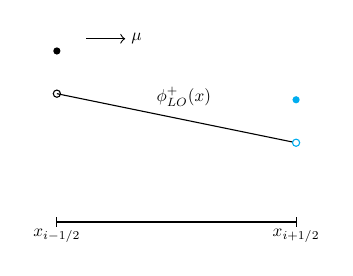
\begin{tikzpicture}[scale=0.62, every node/.style={transform shape}]
            \draw (1.0,4.0) node[fill,circle,inner sep=0pt,minimum
            size=4.2pt] {};
            \draw [->] (1.6,4.25) -- (2.4,4.25) node[anchor=west] {$\mu$};
            \draw (1.0,0.4) -- (1.0,0.6) node[below, pos=0.4] {$x_{i-1/2}$};
            \draw (5.90,0.4) -- (5.90,0.6) node[below, pos=0.4] {$x_{i+1/2}$};
            \node at (3.6,3.06) {$\phi_{LO}^+(x)$};
            \draw [thick] (1.0,0.5) -- (5.9,0.5) node[anchor=north west] {};
            \filldraw[color=black, fill=white] (1,3.1250) circle (2.1pt);
            \draw (1.0,3.125) -- (5.90,2.120);
            \filldraw[color=cyan, fill=white] (5.9,2.120) circle (2.1pt);
            \draw (5.9,3.0) node[cyan,fill,circle,inner sep=0pt,minimum size=4.2pt] {};
        \end{tikzpicture}
    \end{center}
    \caption{Linear doubly-discontinous representation for mean intensity in LO equations}
    \label{fig:ldd_space}
\end{figure}


    Poor statistics for the face tallies may result in this trial space producing less
accurate results compared to the standard LDFE solution, at least for sufficiently fine meshes where LD
can accurately represent the solution.  Although the closure will be applied everywhere,
we expect the greatest improvement in accuracy for cells where the LDFE trial space
produces a negative solution.

By introducing a LDD trial space into the LO equations, we introduce an additional
unknown in each half-range equation.  This extra unknown is eliminated as a function
of the interior moments.  
However, in the HOLO context, the HO solution used a lagged source $q_i$.

In theory, if the problem were linear, or the nonlinear problem was fully converged,
then the HO and LO solutions would produce exactly the same moments.  There are
several issues with ECMC that cause this to not be true, even for a linear problem.
With ECMC, global energy balance is not preserved, but local energy balance is also
not preserved.  There are source biasing techniques for standard MC (systematic
sampling) that would exactly preserve the zeroth moment of the source~\cite{shultis_mc}). 
It is a requirement that the HO solution satisfies the zeroth moment equation. If the
closure relation also uses the first moment, then it must also satisfy the first
spatial moment equation.  However, because we have to reconstruct the bilnear moment
of $x$ and $\mu$, the consistency terms do not exactly preserve the first moment
equation.  One final reason is that the analog treatment of absorption (at low
weights as discussed in Sec.~\ref{???}) results in the fact that the product of
$\phi_i$ (as estimated via path-length estimators) and the removal cross section 
flux does not exactly equal the absorption density of weight within that cell, due to
statistical noise.  
